\section{Results}

\subsection{Synthetic cold splits are already regime-dependent}

We begin with the \texttt{BindingDB\_Kd} synthetic reference panel. Table~\ref{tab:main-results} shows the main pattern: even within a single dataset, model rankings are not stable across split definitions. On \texttt{unseen\_drug}, \texttt{HyperPCM} is strongest by mean \AUPRC{}, reaching $0.5694 \pm 0.0473$ versus $0.5509 \pm 0.0900$ for \texttt{base} and $0.5004 \pm 0.0341$ for \texttt{DTI-LM}. On \texttt{blind\_start}, \texttt{HyperPCM} again has the highest mean \AUPRC{} at $0.3828 \pm 0.1024$, but the margin over \texttt{base} is much smaller and the variance is larger. On \texttt{unseen\_target}, the pattern changes again: \texttt{base} is strongest by mean \AUPRC{} at $0.5224 \pm 0.0602$, while \texttt{DTI-LM} is slightly lower on \AUPRC{} but higher on mean \AUROC{}.

\begin{table}[t]
  \centering
  \scriptsize
  \caption{Synthetic reference panel and promoted real-OOD benchmark. Values are mean $\pm$ std over seeds. Best mean \AUPRC{} in each row is bold.}
  \label{tab:main-results}
  \setlength{\tabcolsep}{3.5pt}
  \resizebox{\linewidth}{!}{
  \begin{tabular}{@{}llcccc@{}}
    \toprule
    Benchmark & Seeds & base (\AUPRC{}/\AUROC{}) & RAICD (\AUPRC{}/\AUROC{}) & FTM sparse (\AUPRC{}/\AUROC{}) & Winner \\
    \midrule
    \texttt{BindingDB\_Kd / unseen\_drug} & 3 &
    \textbf{0.5509 $\pm$ 0.0900 / 0.7794 $\pm$ 0.0534} &
    0.5228 $\pm$ 0.0828 / 0.7803 $\pm$ 0.0506 &
    -- &
    base \\
    \texttt{BindingDB\_Kd / blind\_start} & 3 &
    0.3737 $\pm$ 0.0229 / 0.6778 $\pm$ 0.0151 &
    \textbf{0.4024 $\pm$ 0.0508 / 0.6844 $\pm$ 0.0145} &
    -- &
    RAICD \\
    \texttt{BindingDB\_Kd / unseen\_target} & 3 &
    0.5224 $\pm$ 0.0602 / 0.7741 $\pm$ 0.0161 &
    -- &
    \textbf{0.5439 $\pm$ 0.0791 / 0.7848 $\pm$ 0.0204} &
    FTM \\
    \texttt{BindingDB\_patent / patent\_temporal} & 3 &
    \textbf{0.7772 $\pm$ 0.0086 / 0.7223 $\pm$ 0.0109} &
    0.7692 $\pm$ 0.0018 / 0.7032 $\pm$ 0.0010 &
    0.7721 $\pm$ 0.0025 / 0.7059 $\pm$ 0.0037 &
    base \\
    \bottomrule
  \end{tabular}}
\end{table}


These results matter because they show that ``synthetic cold-start DTI'' is already not a single evaluation condition. Even after replacing internal probes with external literature baselines, different synthetic regimes still reward different model families, so it is unsafe to generalize from one split to another without explicit evidence.

\subsection{Real temporal shift favors a different strong baseline}

We next evaluate the same external panel on \texttt{BindingDB\_patent / patent\_temporal}, our primary real-OOD benchmark. Over three seeds, \texttt{DTI-LM} is the strongest model by mean \AUPRC{}, reaching $0.7825 \pm 0.0078$, compared with $0.7772 \pm 0.0086$ for \texttt{base} and $0.7753 \pm 0.0050$ for \texttt{HyperPCM}. Figure~\ref{fig:delta-summary} compresses the main benchmark story into within-benchmark \AUPRC{} deltas relative to \texttt{base}: synthetic cold splits favor different systems, while the promoted temporal benchmark favors \texttt{DTI-LM}. This temporal advantage is also supported by paired bootstrap: \texttt{DTI-LM - base} $= +0.0054$ with 95\% CI $[+0.0028, +0.0079]$.

\begin{figure}[t]
  \centering
  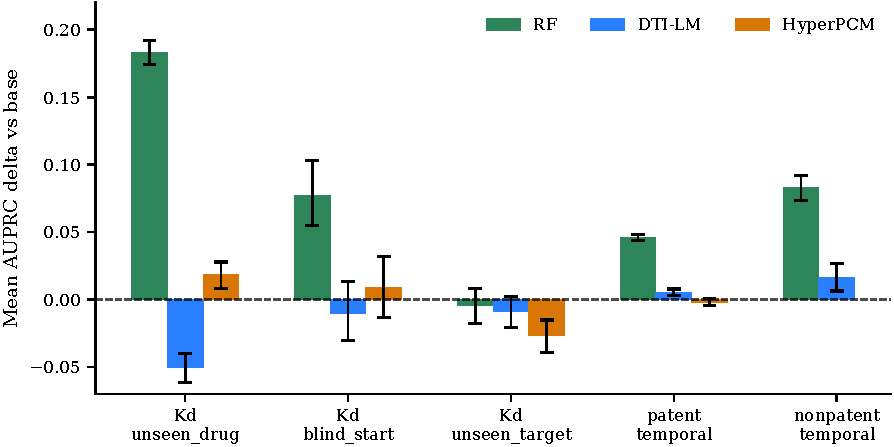
\includegraphics[width=\linewidth]{figures/benchmark_delta_summary.pdf}
  \caption{Mean \AUPRC{} delta relative to \texttt{base} within each benchmark under the external replacement panel. Error bars show paired bootstrap 95\% intervals where available. The synthetic axes and the promoted patent benchmark favor different systems.}
  \label{fig:delta-summary}
\end{figure}

This is the central winner change in the revised paper. The synthetic panel does not produce a single best model, but the promoted temporal benchmark clearly favors \texttt{DTI-LM} by mean \AUPRC{}. The alternative-cutoff benchmark tells the same story over matched three-seed evaluation: on \texttt{patent\_temporal\_v2017}, \texttt{DTI-LM} reaches $0.7134 \pm 0.0027 / 0.6754 \pm 0.0039$, versus $0.7044 \pm 0.0058 / 0.6624 \pm 0.0079$ for \texttt{base}. The broader lesson is therefore not that one external baseline wins everywhere, but that both benchmark axis and model family change the apparent ranking.

\subsection{Temporal shift is structured across year bands and overlap levels}

To help explain why the temporal benchmark changes the ranking, we analyze the patent results by year and by overlap bucket. Table~\ref{tab:patent-diagnosis-compact} makes the primary \AUPRC{} slices explicit, while Figure~\ref{fig:patent-diagnosis} visualizes the same structure. In the large 2019 slice, \texttt{DTI-LM} is strongest by mean \AUPRC{} ($0.7734$), with \texttt{base} ($0.7626$) and \texttt{HyperPCM} ($0.7637$) close behind. In 2020, however, the ordering flips: \texttt{base} reaches $0.8715 / 0.8135$, while \texttt{DTI-LM} and \texttt{HyperPCM} drop to $0.8545 / 0.7951$ and $0.8526 / 0.7938$, respectively. The 2021 slice is small, but again strongly favors \texttt{base}.

The overlap-bucket analysis reveals another useful pattern. In the lowest-overlap bucket, \texttt{DTI-LM} is strongest by mean \AUPRC{} ($0.6353$), while \texttt{HyperPCM} is close behind. In the middle-overlap bucket, \texttt{HyperPCM} takes a small lead on \AUPRC{} ($0.7513$) over \texttt{DTI-LM} ($0.7489$) and \texttt{base} ($0.7218$). In the highest-overlap bucket, the ordering flips again and \texttt{base} dominates on both \AUPRC{} and \AUROC{}. Together, these results are consistent with the view that temporal OOD is not just a colder version of synthetic cold-start. Instead, it changes which subpopulations dominate the aggregate result, and therefore changes the model ranking.

\begin{table}[t]
  \centering
  \scriptsize
  \caption{Compact \AUPRC{} summary behind the patent diagnosis under the external replacement panel. Values are mean $\pm$ seed std over the matched 3-seed runs. The tiny 2021 slice is pooled into the \texttt{2020--2021} stratum to avoid over-interpreting a 72-example cell.}
  \label{tab:patent-diagnosis-compact}
  \setlength{\tabcolsep}{3.5pt}
  \resizebox{\linewidth}{!}{
  \begin{tabular}{@{}llcccc@{}}
    \toprule
    Slice type & Slice & Count & base & DTI-LM & HyperPCM \\
    \midrule
    Year & 2019 & 42,009 & 0.7626 $\pm$ 0.0098 & \textbf{0.7734 $\pm$ 0.0071} & 0.7637 $\pm$ 0.0049 \\
    Year & 2020--2021 & 7,019 & \textbf{0.8716 $\pm$ 0.0121} & 0.8533 $\pm$ 0.0100 & 0.8516 $\pm$ 0.0139 \\
    Overlap bucket & 0 ($0.000$--$0.531$) & 16,341 & 0.5551 $\pm$ 0.0190 & \textbf{0.6353 $\pm$ 0.0175} & 0.6147 $\pm$ 0.0208 \\
    Overlap bucket & 1 ($0.531$--$0.710$) & 16,342 & 0.7218 $\pm$ 0.0167 & 0.7489 $\pm$ 0.0094 & \textbf{0.7513 $\pm$ 0.0060} \\
    Overlap bucket & 2 ($0.710$--$0.989$) & 16,345 & \textbf{0.9237 $\pm$ 0.0030} & 0.8866 $\pm$ 0.0097 & 0.8767 $\pm$ 0.0042 \\
    \bottomrule
  \end{tabular}}
\end{table}


\begin{figure}[t]
  \centering
  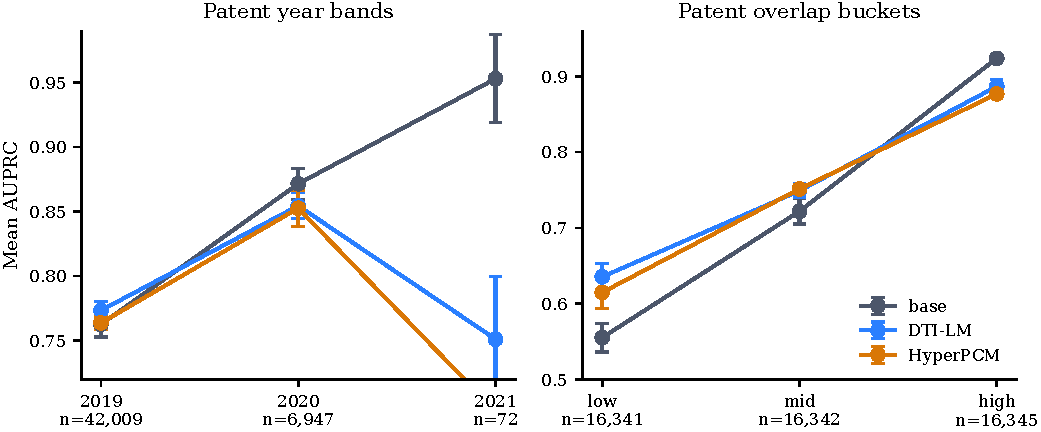
\includegraphics[width=\linewidth]{figures/patent_shift_diagnosis.pdf}
  \caption{Patent temporal diagnosis in terms of mean \AUPRC{} under the external replacement panel. Left: year-band slices. Right: test-set overlap buckets computed from the saved overlap score. The aggregate \texttt{DTI-LM} advantage is concentrated in the 2019 and lower-overlap strata, while \texttt{base} dominates the 2020 and highest-overlap slices.}
  \label{fig:patent-diagnosis}
\end{figure}

\subsection{Supporting target-cold OOD benchmarks still favor the plain base model}

We treat \texttt{BindingDB\_Ki / unseen\_target} and \texttt{DAVIS / unseen\_target} as supporting real-OOD benchmarks rather than primary headline axes. Under matched three-seed evaluation, neither promoted external baseline overturns the support-panel story. On \texttt{BindingDB\_Ki}, \texttt{base} reaches $0.6934 \pm 0.0257 / 0.7192 \pm 0.0068$, compared with $0.6648 \pm 0.0177 / 0.6936 \pm 0.0044$ for \texttt{DTI-LM} and $0.6515 \pm 0.0301 / 0.6757 \pm 0.0211$ for \texttt{HyperPCM}. On \texttt{DAVIS}, \texttt{base} reaches $0.4097 \pm 0.0275 / 0.8613 \pm 0.0153$, compared with $0.4090 \pm 0.0570 / 0.8718 \pm 0.0152$ for \texttt{DTI-LM} and $0.3840 \pm 0.0269 / 0.8610 \pm 0.0245$ for \texttt{HyperPCM}.

The \texttt{DAVIS} result is the closest supporting-panel case: \texttt{DTI-LM} is effectively tied with \texttt{base} on mean \AUPRC{} and slightly higher on mean \AUROC{}, but it still does not create a clean winner change of the kind seen on the promoted patent benchmark. \texttt{BindingDB\_Ki} is more decisive, with \texttt{base} ahead of both external baselines on both metrics. These auxiliary results are therefore consistent with the main claim of the paper, but they do not carry the same argumentative weight as the patent benchmark because they do not add a cleaner ranking-reversal axis than temporal/provenance shift.
